\documentclass[../main.tex]{subfiles}

\begin{document}

%%%%%%%%%%%%%%%%%%%%%%%%%%%%%%%%%%%%%%%%%%%%%%%%%%%%%%%%%%%%%%%%%%%%%%%%%%%%%%%
%%%%%%%%%%%%%%%%%%%%%%%%%%%%%%%%%%%%%%%%%%%%%%%%%%%%%%%%%%%%%%%%%%%%%%%%%%%%%%%
\section{Building models, but at what cost?}
\label{sec:building_models_but_at_what_cost_}
%%%%%%%%%%%%%%%%%%%%%%%%%%%%%%%%%%%%%%%%%%%%%%%%%%%%%%%%%%%%%%%%%%%%%%%%%%%%%%%
%%%%%%%%%%%%%%%%%%%%%%%%%%%%%%%%%%%%%%%%%%%%%%%%%%%%%%%%%%%%%%%%%%%%%%%%%%%%%%%

Supervised learning uses a cost function that we aim to minimize.
However, minimizing such functions with the data available can sometimes be
costly both in term of time and memory.
In a regression setting, the popular least-squares estimator benefits from great
interpretability.
For a response $y\in\bbR^n$ and some data $X\in\bbR^{n\times p}$ a least-squares
estimator $\hat\beta^{\mathrm ls}$ is any solution of the optimization problem:
\begin{align*}
\hat\beta^{\mathrm ls}
\in
\argmin_{\beta\in\bbR^p}\frac{1}{2n}\norm{y-X\beta}_2^2\enspace.
\end{align*}
Some issues can arise like the curse of dimensionality.
When $p$ is larger than $n$, uniqueness of the solution is lost,
leading to non interpretable coefficients.
For this reason, penalties can be added to the cost function to recover targeted
structures.
We focus on the Elastic-Net \citep{Zou_Hastie05} estimator $\hat\beta^{\mathrm en}$.
It uses a trade-off between the $\ell_1$ (LASSO \citep{Tibshirani96})
and $\ell_2$ (Ridge \citep{Tikhonov43}) penalties on the coefficients to induce
sparsity and regularize the problem.
We remind that the $\ell_1$ norm is the sum of the magnitude of the
coefficients and the squared $\ell_2$ norm is the sum of squares of the coefficients.
The Elastic-Net is thus
\begin{align}\label{eq:classic_enet}
\hat\beta^{\mathrm en}
\in
\argmin_{\beta \in \bbR^p}
 \frac{1}{2n} \norm{y - X\beta}_2^2
+ \lambda_{\ell_1} \norm{\beta}_1
+ \frac{\lambda_{\ell_2}}{2} \norm{\beta}_2^2\enspace.
\end{align}
In our model, we want to handle first order interactions.
To do so, we have to consider a matrix $Z$ whose columns are involving a function
that creates new covariates from couples of original data.
This function in all generality could be a $\max$, $\min$,\dots.
We chose to focus on the element-wise product.
This is not the most interpretable for biologists, but it creates a base that is
easy to implement and easy to modify afterwards for new functions.
More practically, it means that $Z$ has $n$ samples and $d$ features with $d$
the number of unique interactions.
As for the estimation, in addition to the vector $\beta\in\bbR^p$, we need to
estimate a vector $\Theta\in\bbR^{d}$.
For the $1^{st}$ feature there are $p$ other features to interact with, $(p-1)$
for the $2^{nd}$,\dots, two for the $(p-1)^{th}$ and one for the last.
So in total there are $d=\nicefrac{p(p+1)}{2}$ unique interactions to consider.

\medskip

The memory footprint of $Z$ is in practice quickly too large for
the computer.
From \Cref{fig:size_matrix}, we see that the memory footprint of $Z$ with $500$
features and $20000$ samples in $X$ exceeds $10$Gb.
So there are difficulties not only for the statistics part, but also for
the implementation of the solvers.
 \begin{figure}[h!]
    \centering
    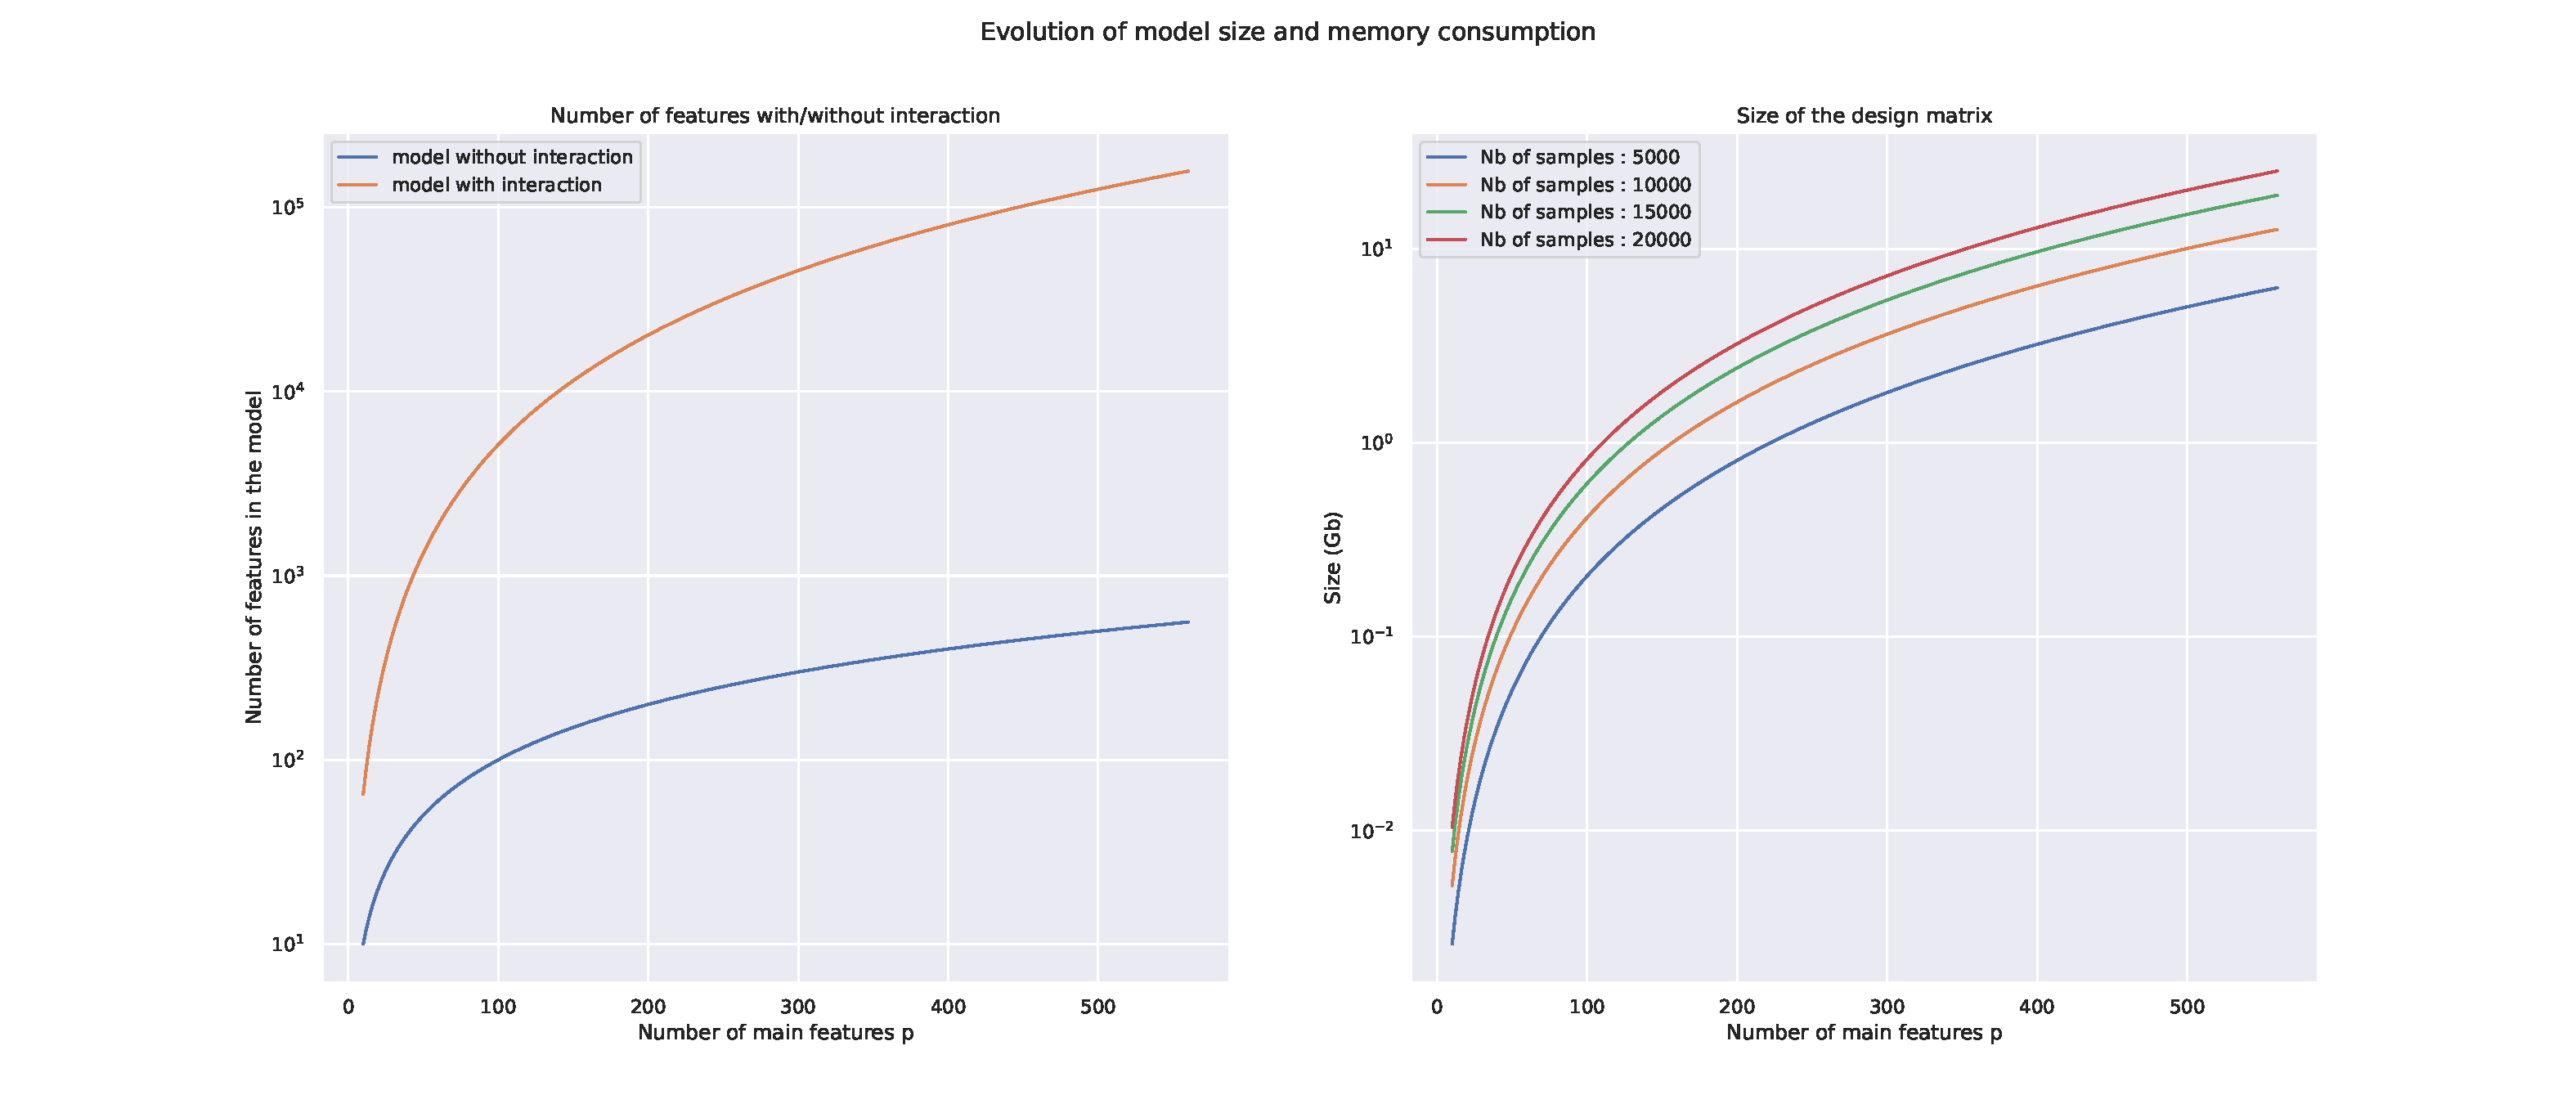
\includegraphics[scale=.45]{size_matrix.pdf}
    \caption{Number of features in the models with and without
    interactions (left) and size of the interaction matrix in Gigabytes for
    varying number of features in $X$ (right).}
    \label{fig:size_matrix}
\end{figure}

\medskip

Research for fast algorithms to solve Elastic-Net or LASSO problems is very
active.
These problems search for the active variables \ie without interactions
$\{\beta_i:\beta_i\neq 0,\ i=1,\dots,p\}.$
Some strategies like the working set are to build up the support by
including features that are likely active \citep{johnson2015blitz}.
Other methods (safely) discard features that are not relevant using the duality gap
\citep{ndiaye2017gap}.
Solvers can also be accelerated.
Inertial acceleration like Nesterov \citep{nesterov2012efficiency}
lead to theoretically faster methods (but sometimes not in practice).
Anderson extropolation \citep{bertrand2021anderson} can also be used.
It is not an inertial acceleration but considers the structure of the iterates to
converge faster.
Stochastic methods are also used to determine the direction to optimize
\citep{chen2021global}.

\medskip

On top of the theoretical accelerations, libraries like \texttt{Numba}
\citep{lam2015numba} lead to some computational speed up.
This is what is used in \citep{Bascou_Lebre_Salmon20} to solve the Elastic-Net
with interactions.
In our work, we propose to use the GPU with inertial acceleration.
%%%%%%%%%%%%%%%%%%%%%%%%%%%%%%%%%%%%%%%%%%%%%%%%%%%%%%%%%%%%%%%%%%%%%%%%%%%%%%%
%%%%%%%%%%%%%%%%%%%%%%%%%%%%%%%%%%%%%%%%%%%%%%%%%%%%%%%%%%%%%%%%%%%%%%%%%%%%%%%
\section{Computation with a GPU}
\label{sec:exploiting_the_power_of_the_graphic_card}
%%%%%%%%%%%%%%%%%%%%%%%%%%%%%%%%%%%%%%%%%%%%%%%%%%%%%%%%%%%%%%%%%%%%%%%%%%%%%%%
%%%%%%%%%%%%%%%%%%%%%%%%%%%%%%%%%%%%%%%%%%%%%%%%%%%%%%%%%%%%%%%%%%%%%%%%%%%%%%%
With the rise of new technologies for always better graphical rendering in
video games, graphics cards have become a computational powerhouse.
Generally, computations are made on CPUs (Central Processing Unit).
Standard programs are designed for them, so there is no extra manipulation
needed.
This is different for GPUs (Graphic Processing Unit).
\begin{figure}[h]
    \centering
    \def\svgscale{0.35}
    \includesvg{./sources_images/GPU_diag}
    \caption{Simplified architecture of a GPU adapted from \citep[chapter 2]{feydy2020fast}.
    Typically, the data is first loaded onto the CPU.
    Then it is \textcolor{darkgreen}{copied (sometimes in part) to the GPU device}.
    This operation is very costly.
    There is a hierarchy of memory from here.
    Each GPU has an L2 cache which communicates with several independant L1
    caches for each block.
    Threads operations are then executed simultaneously, organized in blocks.
    After all operations are done,
    the results are \textcolor{red}{transferred back to the CPU}.
    }
    \label{fig:GPU_intro}
\end{figure}

A GPU has a very large amount of cores allowing heavy parallelizations,
possibly asynchronously (see \Cref{fig:GPU_intro}).
This means that operations are kept in a queue and computed when needed.
In the corporate world of GPUs, there is mostly only NVidia that is
investing for faster devices for the AI research.
They have developed the \texttt{CUDA} toolkit for developers to leverage GPUs
performances.
At first code in \texttt{C} / \texttt{C++}, libraries like \texttt{PyTorch},
\texttt{TensorFlow} in \texttt{Python} or \texttt{RCUDA} in \texttt{R}
created APIs to use \texttt{CUDA} acceleration more easily.

\medskip

There are some changes that need to be addressed with GPUs.
Some of them are discussed in \Cref{chap:an}.
But one (if not the main) to remember, is that transfers between CPUs and GPUs
are usually creating the computation bottleneck.
Transferring data from one device to another is very costly.
So even if $Z$ was storable on the CPU, making transfers to the GPU by parts
would be very slow.

%%%%%%%%%%%%%%%%%%%%%%%%%%%%%%%%%%%%%%%%%%%%%%%%%%%%%%%%%%%%%%%%%%%%%%%%%%%%%%%
%%%%%%%%%%%%%%%%%%%%%%%%%%%%%%%%%%%%%%%%%%%%%%%%%%%%%%%%%%%%%%%%%%%%%%%%%%%%%%%
\section{Leveraging GPUs computations for the optimization}
\label{sec:levering_gpus_computations_for_optimization}
%%%%%%%%%%%%%%%%%%%%%%%%%%%%%%%%%%%%%%%%%%%%%%%%%%%%%%%%%%%%%%%%%%%%%%%%%%%%%%%
%%%%%%%%%%%%%%%%%%%%%%%%%%%%%%%%%%%%%%%%%%%%%%%%%%%%%%%%%%%%%%%%%%%%%%%%%%%%%%%

State-of-the-art solvers consider coordinate descent type algorithms for sparse
regression.
The strength of the GPU comes from the possibility to process a lot of data
simultaneously.
These algorithms treat each feature separately, so very few data at a time.
Our goal is thus to determine if some methods generally slow on CPUs could be
competitive using \texttt{CUDA} acceleration.
After presenting the (proximal) gradient descent methods
we will explore some pros and cons of using GPUs in such settings.
Then we apply our solvers to simulated datasets and a real genomics dataset to
explore different behaviors.
One of the difficulties encountered when dealing with such algorithms is the
convergence.
Indeed, we need a stopping criterion in order to decide when the convergence
is reached.
For that, we derive the KKT violation criterion for the Elastic-Net with
interactions.

\medskip

This work was made during an internship supervised by
Joseph Salmon\footnote{\url{http://josephsalmon.eu/}} and
Benjamin Charlier\footnote{\url{https://imag.umontpellier.fr/~charlier}}
at the Institut Montpellierain Alexender Grothendieck.
The base material is from the ongoing work of Florent Bascou\footnote{\url{https://bascouflorent.github.io/}}.
The genomics dataset was provided by Sophie Lèbre\footnote{\url{https://www.univ-montp3.fr/miap/~lebre/}}.

\end{document}
